% ВАЖНО
% Не меняйте ничего в этом файле. А если меняете, то делайте это в этом проекте:
% https://github.com/kib-courses/latex_templates
% Для пользовательских настроек есть файл ./header/user.tex
\documentclass{beamer}
\usetheme{metropolis} 
\usecolortheme{rose}

\hypersetup{unicode=true}
\usepackage{tikz}

\usepackage{xcolor}
\usepackage[utf8]{inputenc}
\usepackage{hyphenat}
\usepackage[russian,english]{babel}          % Use metropolis theme
\usepackage{wrapfig}

\usepackage[normalem]{ulem}  % для зачекивания текста

\usepackage{caption}
\captionsetup[figure]{name=Рисунок }
\newcommand{\рис}[1]{рис.\ref{#1}}
\newcommand{\Рис}[1]{Рис.\ref{#1}}


\captionsetup[table]{name=Таблица~№}
\newcommand{\таблицa}[1]{таблица~№\ref{#1}} % именительный падеж
\newcommand{\таблицы}[1]{таблицы~№\ref{#1}} % родительный падеж
\newcommand{\таблице}[1]{таблице~№\ref{#1}} % дательный и предложный падеж
\newcommand{\таблицу}[1]{таблицу~№\ref{#1}} % винительный падеж
\newcommand{\таблицей}[1]{таблицей~№\ref{#1}} % творительный падеж 
\newcommand{\Таблицa}[1]{Таблица~№\ref{#1}} % именительный падеж
\newcommand{\Таблицы}[1]{Таблицы~№\ref{#1}} % родительный падеж
\newcommand{\Таблице}[1]{Таблице~№\ref{#1}} % дательный и предложный падеж
\newcommand{\Таблицу}[1]{Таблицу~№\ref{#1}} % винительный падеж
\newcommand{\Таблицей}[1]{Таблицей~№\ref{#1}} % творительный падеж 

\setbeamertemplate{footline}[frame number] % указывает на каждой странице общее количество страниц

% Указывайте все новые термины в \termdef команде. А уже известные ранее или из других курсов в \term
\newcommand{\termdef}[1]{\textbf{\textit{#1}}}
\newcommand{\term}{\textit}

% Диалог с аудиторией.
\newcommand{\auditorium}[1]{\textcolor{red}{\textbf{#1}}}

\let\OLDhref\href
\renewcommand{\href}[2]{\textcolor{blue}{\OLDhref{#1}{#2}}}

% \setbeameroption{show notes}
% \usepackage{listings}             % Include the listings-package
% \usepackage{minted}

\usepackage{CJKutf8}

\title{Лекция 6. UEBA: алгоритмы <<behс>> и <<behi>>. Обнаружение социальной инженерии. Задача распознавания семейства ВПО.}

% \date{\today}
\date{12 ноября 2019}
\author{Павел Владимирович Слипенчук }
\institute{Москва, МГТУ им.Бауманка,\\ каф.ИУ-8, \href{https://t.me/kibinfo}{КИБ}}
% \titlegraphic{\includegraphics[width=2cm]{logo_ur.jpg}}
\titlegraphic{\small \href{https://github.com/kib-courses/dsis}{Data Science для решения задач информационной безопасности}}

\begin{document}
  \maketitle
    
\begin{frame}{План лекции}
    \begin{enumerate}
    	\item \nameref{section:nn_no_work}
		\item \nameref{section:text_tasks}
		\item \nameref{section:behс}
		\item \nameref{section:behi}
	\end{enumerate}
\end{frame}

\section{Как НЕ работают нейронные сети}\label{section:nn_no_work}
% прерывные потоки и почему не работает нейронные сети

\begin{frame}
	\small
	Нейронная сеть -- это последовательно-параллельный ансамбль решающих пней.
	
	\begin{center}
		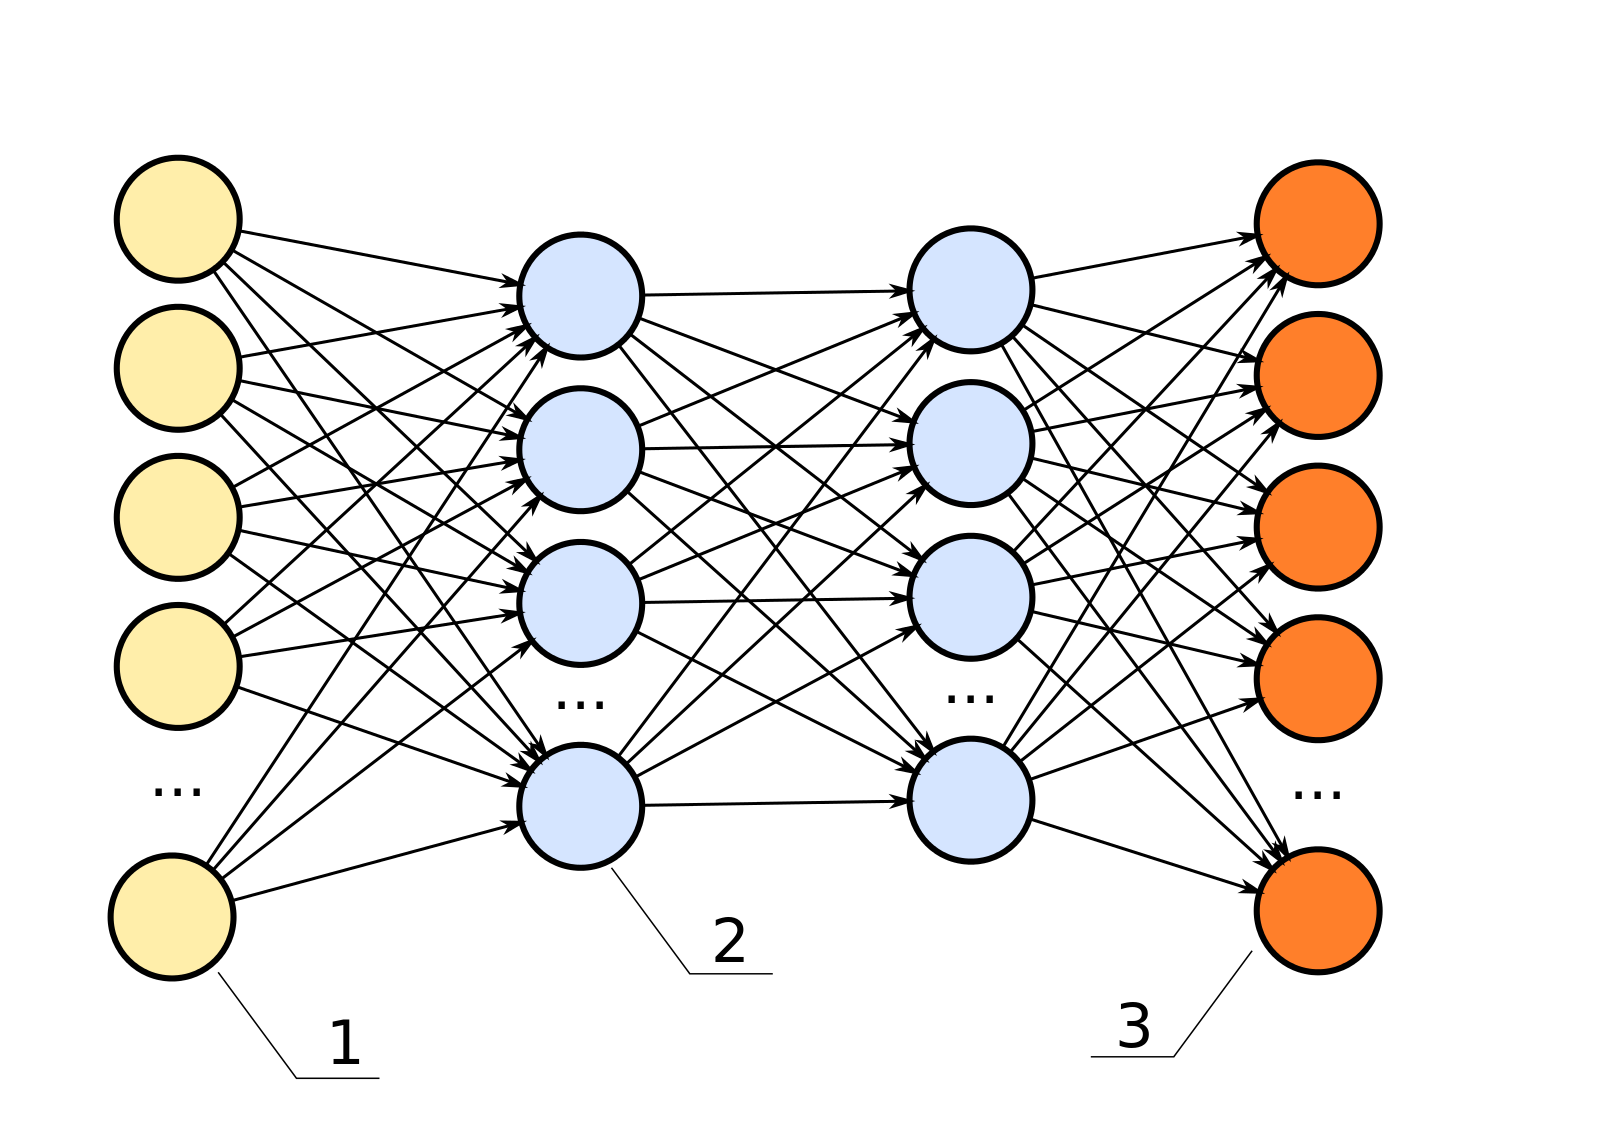
\includegraphics[width=7.5cm]{../pic/nn_example.png}\centering
	\end{center}
	
	Любую ЭС можно представить как нейронную сеть.
	
	Проблема нейронных сетей -- как их обучать.
\end{frame}

\begin{frame}{Backpropagation}
	Метод обратного распространения ошибки (backpropagation) 
	-- требует <<локальной связности>> признаков. 
	
	Изображение (пиксели), временные ряды, треки мыши, голос этой <<локальной связностью>>
	обладают.
	
	Текст естественного языка -- в меньшей степени. Но текстов очень много и букв всего 33.
\end{frame}

\begin{frame}{Проблема больших алфавитов и разряженных слов}
	
	Представьте себе цепочки с алфавитом в 300-500 букв,
	которые достаточно разряжены.
	
	TODO изображение.
	
	Теоретически их тоже можно решить нейронной сетью,
	однако потребуется большее количество данных, чем для текста.
\end{frame}


\section{Постановка задач ИБ}\label{section:text_tasks}


\section{Алгоритм behс}\label{section:behс}


\section{Алгоритм behi}\label{section:behi}


\section{Вопросы для самопроверки}

\end{document}